\chapter{Analyse}

\section{Objectifs principaux}

La mise en place et la prise en main de la librairie OpenCV ont été sousestimées.
En effet, comme nous n'avions jamais utilisé cette librairie auparavant, nous ne connaissions pas exactement les possibilités qui s'offraient à nous.
Lors de l'implémentation, nous nous sommes rendus compte que certains objectifs étaient hors-sujets, trop complexes à mettre en place, ou simplement infaisables avec OpenCV.
C'est pourquoi ceux-ci, sous l'accord de M Beurret, ont été mis à jour tout au long de ce projet.


Le premier point sera de récupérer un flux vidéo capturé en direct (webcam, appareil photo ou caméra) et de l'afficher tel quel.
Un autre objectif sera de permettre à l'utilisateur de prendre des instantanés du rendu vidéo et de l'enregistrer au format PNG.
De plus, nous souhaitons offrir à l'utilisateur la possibilité de modifier le rendu vidéo en temps réel et ce par le biais de différents panels de réglages identifiés par les thèmes suivants : Colorimétrie, Filtres, Effets spéciaux et Animations.
Les deux premières catégories seront composées de slider, de spinbox et de boutons, comme illustré dans la Figure \ref{maquette_parametres}. 
Tous les réglages pourront être réalisés et appliqués simultanément.
Les deux catégories suivantes, quant à elles, seront représentées comme dans la Figure \ref{maquette_animation}.
L'utilisateur ne pourra utiliser qu'un seul effet spécial à la fois mais pourra cumuler autant d'animations qu'il le souhaite.

\begin{figure}[h]
  \centering
  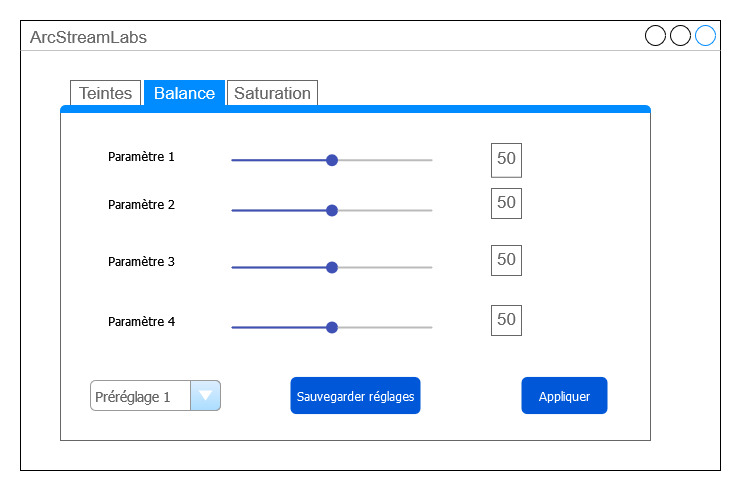
\includegraphics[width=\textwidth]{./images/P2_Maquette_Parametres.jpg}
  \caption{Maquette des paramètres}
  \label{maquette_parametres}
\end{figure}

\begin{figure}[h]
  \centering
  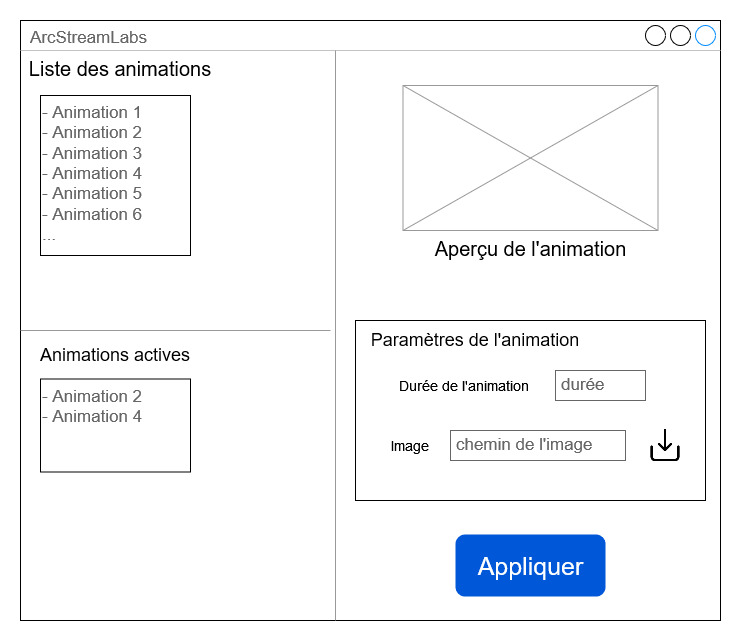
\includegraphics[width=\textwidth]{./images/P2_Maquette_Animations.jpg}
  \caption{Maquette des animations}
  \label{maquette_animation}
\end{figure}

\subsection{Colorimétrie}

La colorimétrie permettra de retravailler le rendu visuel de l'image à proprement parlée. Celle-ci comprendra :

\textbf{ Principaux : }

\begin{itemize}
  \item Balance des couleurs;
  \item Exposition;
  \item Gestion des tons (sombre / clair);
  \item Luminosité ainsi que le contraste
  \item saturation
  \item Température des couleurs
  \item Teinte chromatique
  \item Teinte de saturation
\end{itemize}

\textbf{ Optionnels : }

\begin{itemize}
  \item Travail par courbe
  \item Travail par niveau
\end{itemize}

\subsection{Filtres}

Les filtres permettront d'appliquer une liste d'effets en complément des réglages colorimétriques, tels que :

\begin{itemize}
  \item Filtre 'Sobel'
  \item Filtre 'Exposure'
  \item Filtre 'Stylization'
\end{itemize}

\subsection{Effets spéciaux}

Les effets spéciaux viendront donner un corps à la modification de la vidéo en transformant significativement cette dernière.

\begin{itemize}
  \item Mirroring (Inversion sur l'axe vertical)
  \item Mosaic blur (floutage sous forme de mosaïque)
  \item Détection faciale + Floutage
\end{itemize}

\subsection{Animations}

Les animations seront des additions d'éléments externes à la vidéo.
Il y en aura principalement deux types.
Le premier sera de faire bouger une ou plusieurs icônes de 40x40 pixels en suivant des patterns définis ou aléatoires.

\begin{itemize}
  \item Détection faciale (bouche) + Superposition d'une image de moustache
  \item Bouncing text (Logo DVD)
\end{itemize}

Le deuxième sera l'utilisation de gifs laissés au choix de l'utilisateur.

\textbf{ Principaux : }

\begin{itemize}
  \item Entrée de champs (point d'entrée défini par l'utilisateur)
  \item Fondu
  \item Traversant
\end{itemize} 

\section{Objectifs secondaires}

Au travers de ce projet, nous souhaitons devenir plus intime avec le concept d'expérience utilisateur.
Dans un tout autre registre, nous voulons nous confronter à la problématique des ralentis, l'idée est de réussir à avoir un ralenti sans pour autant augmenter le délai capture/diffusion.
Finalement, nous souhaitons explorer notre créativité au travers d'ajout de filtres et d'effets spéciaux.

\section{Objectifs tertiaires}

Si le temps nous le permets nous aimerions également pouvoir nous pencher sur le travail du son, ajout d'une soundboard mais aussi applications de divers filtres sonores.

\newpage

\begin{landscape}

\section{Planification initiale}

\begin{figure}[h]
  \centering
  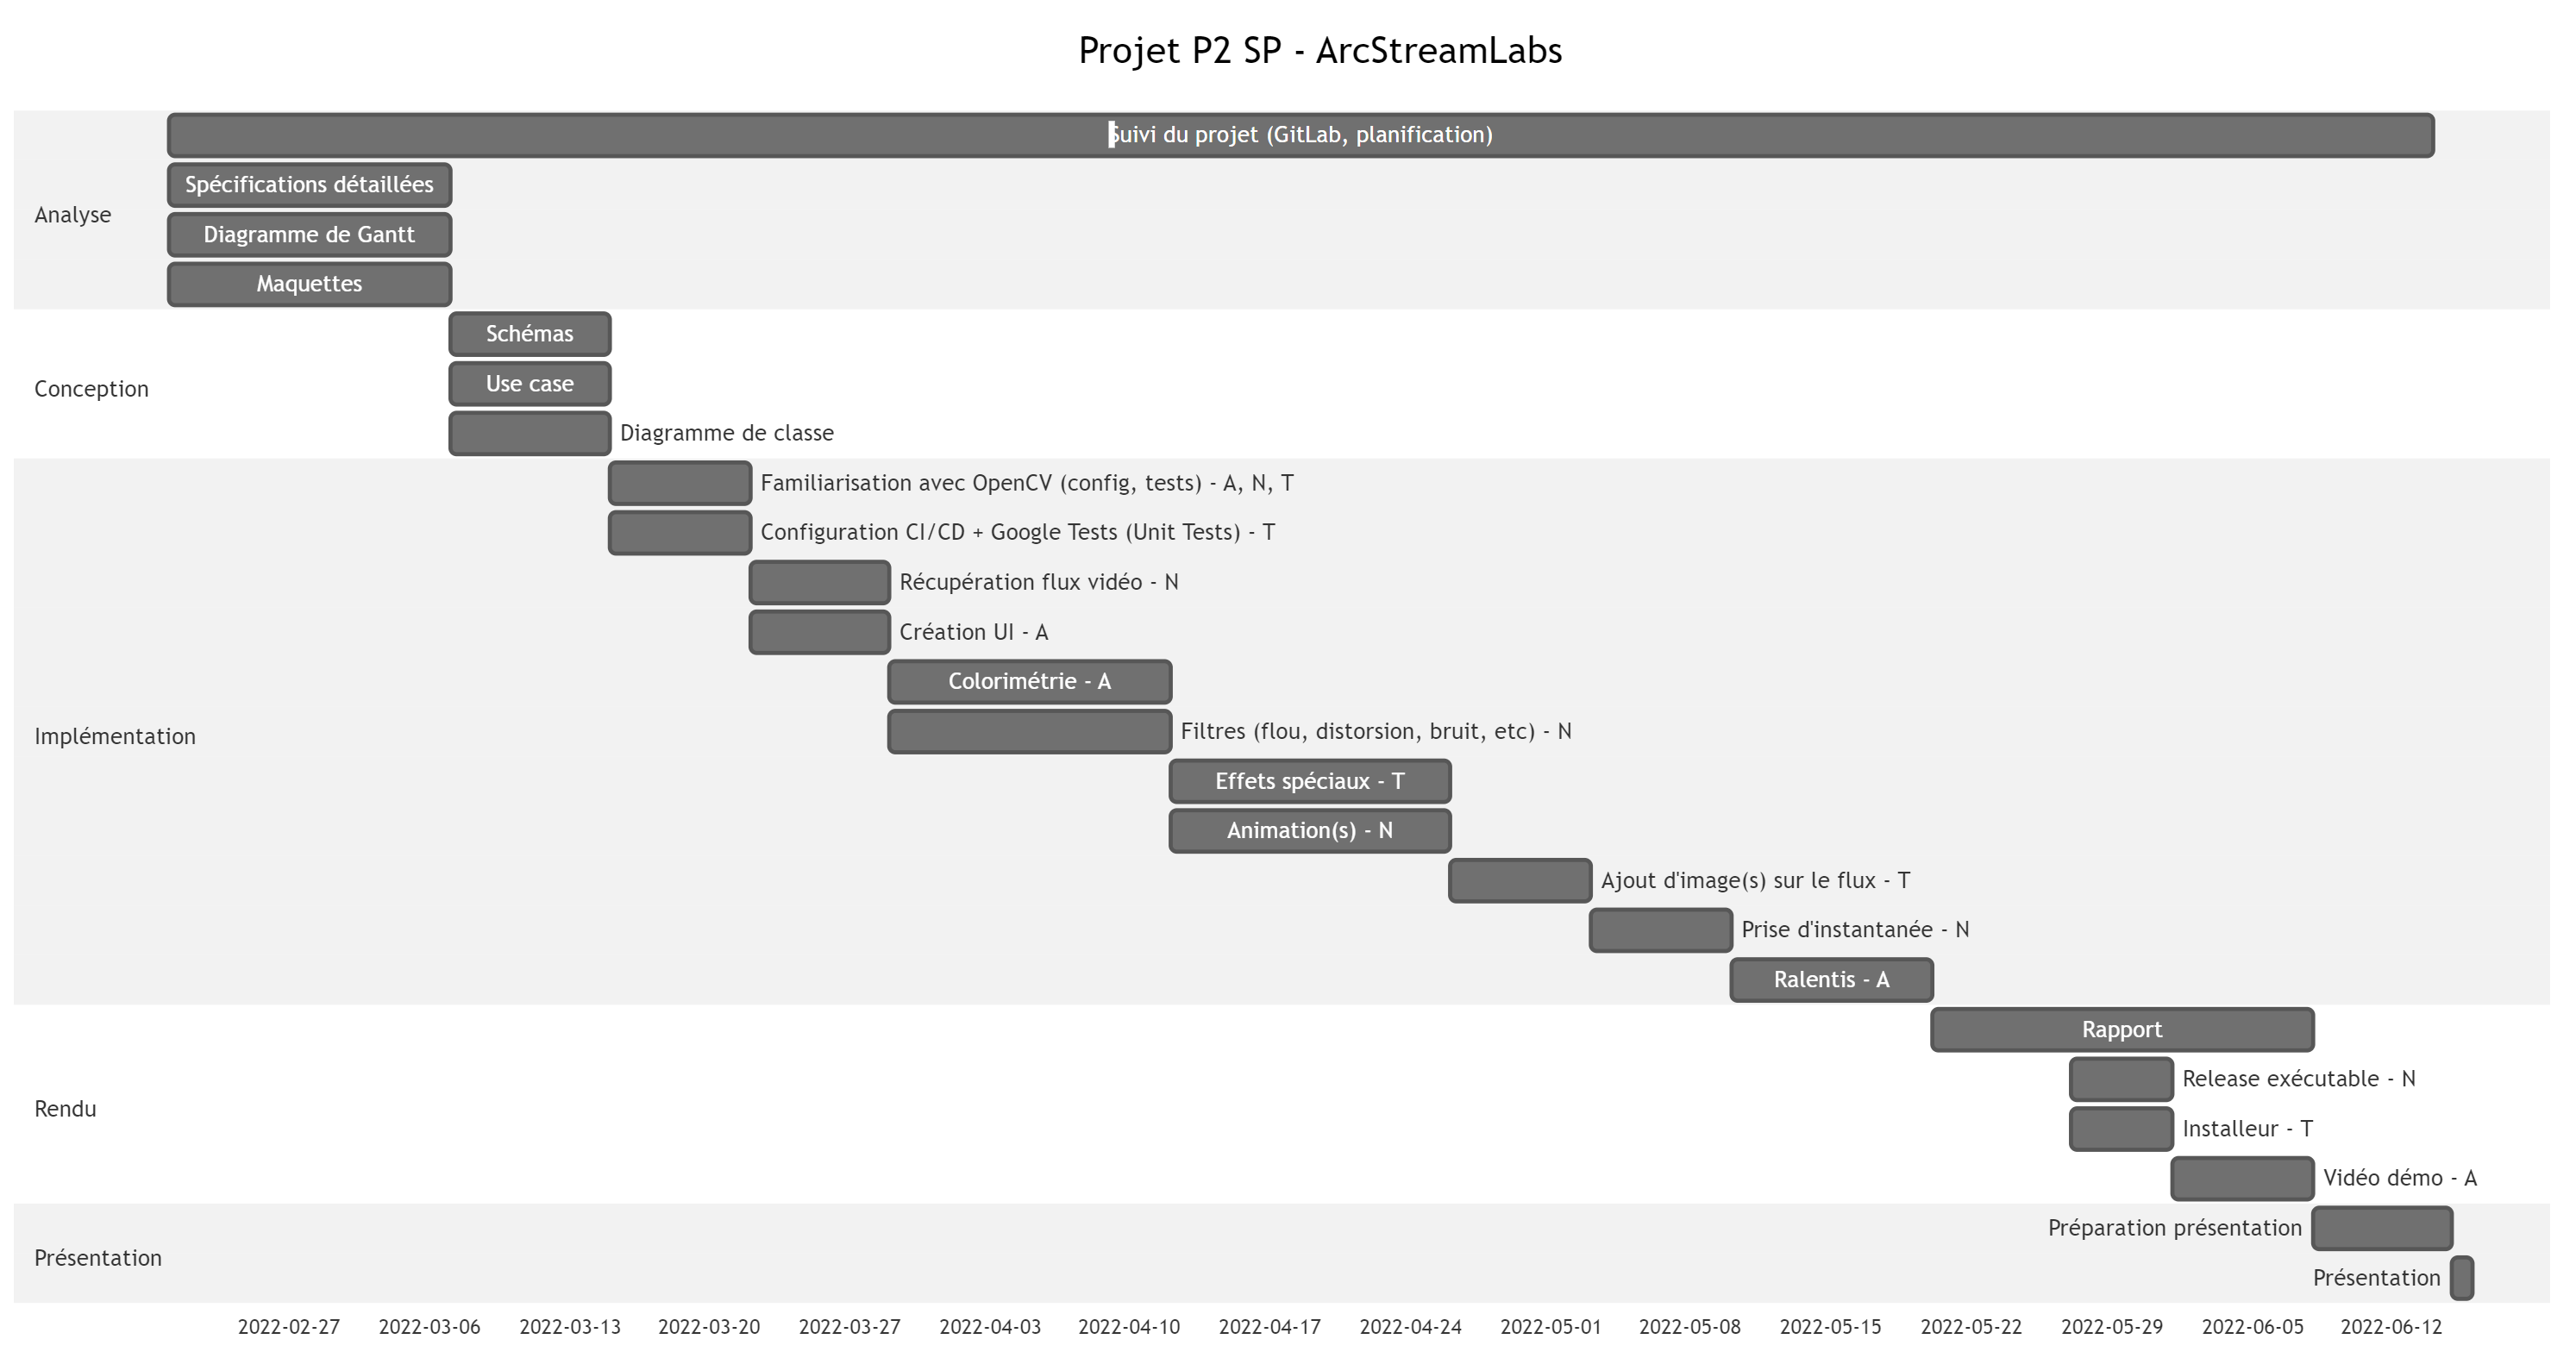
\includegraphics[width=\textwidth]{./images/gantt.PNG}
  \caption{Planification GANTT}
  \label{gantt}
\end{figure}

\end{landscape}

\newpage

\begin{landscape}

\section{Diagramme des cas d'utilisation}

\begin{figure}[h]
  \centering
  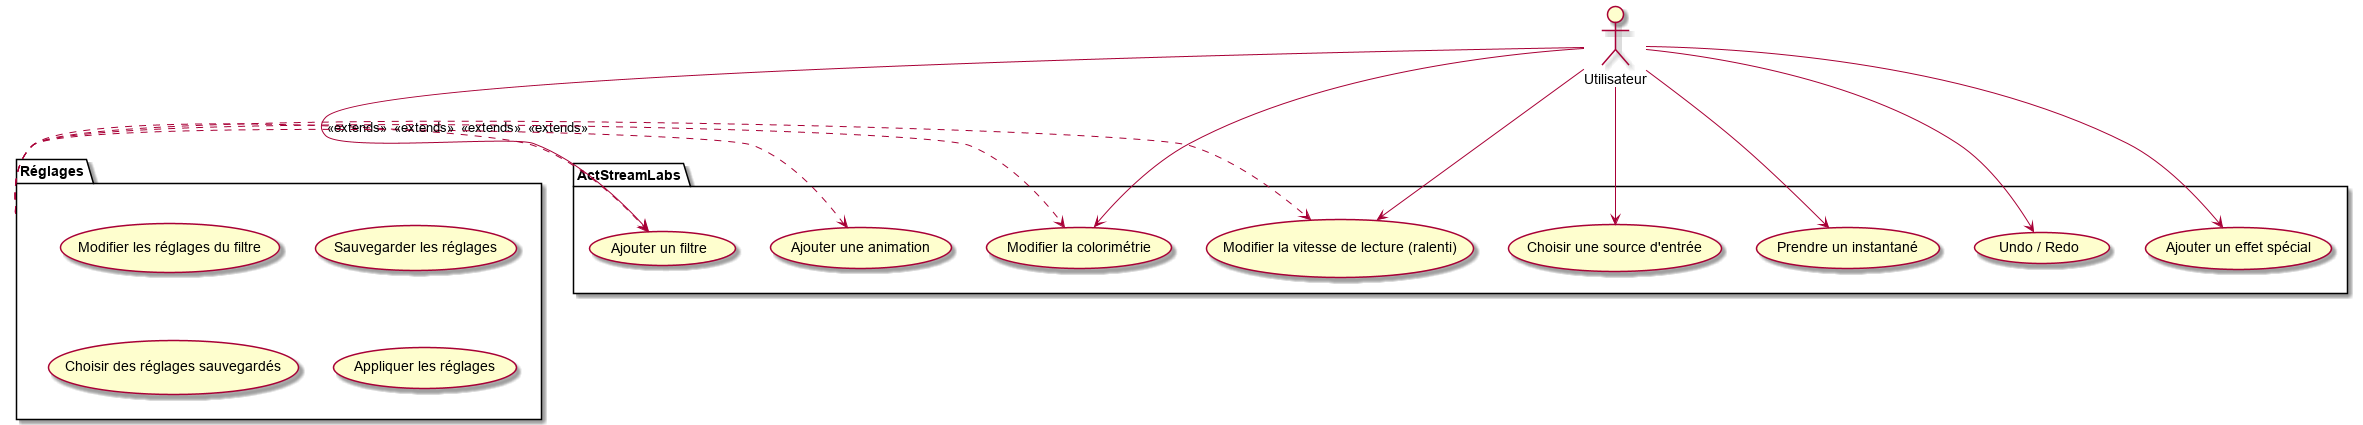
\includegraphics[width=\textheight]{./images/useCase.png}
  \caption{Diagramme des cas d'utilisation}
  \label{useCase}
\end{figure}

\end{landscape}

\section{Technologies utilisées}

\textcolor{red}
{
Il faut détailler le context du projet, les besoins, les spécifications, etc.
Quelle est la motivation derrière ce projet ?
Qu'est-ce que ce projet apportera au final ?
On peut rajouter un diagramme WBS pour donner un aperçu haut-niveau :
}

Afin de mettre en pratique les connaissances acquises lors du cours de Génie Logiciel dispensé par M Le Callenec,
il nous a été demandé d'intégrer au moins un structure de données complexe à notre projet.

Certains filtres demanderont des traitements assez lourds ; ceux-ci pourront entraîner des délais entre le flux entrant (capturé) et le flux sortant (affiché à l'utilisateur).
Afin de limiter de nombre d'images (de frames en attente de traitement) stocké par notre application, nous allons mettre en place un buffer circulaire.

Puis, dans le but d'améliorer l'expérience utilisateur ainsi que pour approfondir nos capacités de conception, nous essaierons de concevoir et d'implémenter un mécanisme d'Undo / Redo.

\section{Faisabilité}

\textcolor{red} 
{
Quels sont les contraintes de ce projet ? En quoi elles sont surmontables ? Un preuve de concept existe-t'elle déjà ?
}

\section{Risques}
\textcolor{red} 
{
  Faire une analyse de risques et donner les solutions envisagées le cas échéant.
  Pour chaque risque, il faut détailler les informations suivantes :
  \begin{itemize}
    \item Son numéro;
    \item Son nom;
    \item Sa description;
    \item Sa probabilité : très improbable, improbable, probable, très probable;
    \item Son impact :  faible, modéré, grave, très grave;
    \item Niveau de criticité (Probabilité * Impact)
    \item Les mesures de prévention
    \item Les mesure de correction
  \end{itemize}
}

Ensuite, on peut résumer ces informations dans un tableau comme ce qui suit :

\begin{tabular}{ | l | l | l | l | }
  N° & Nom & Probabilité & Impact \\
  \rowcolor{red!60}
  01 & Risque critique & probable & grave \\
  \rowcolor{red!20}
  02 & Risque acceptable & probable & faible \\
  03 & Risque insignifiant & peu probable & faible
\end{tabular}
